The kalman filter is a method for sensor fusion. It is capable of taking two or more measurements and fuse together to one optimal guess of the true value. It does this by looking at the current measurement and comparing it with a predicted value. The predicted value is often a combination of the previous value combined with the changed done since the last measurement. 

The kalman filter has some limitations. One of them is that it assume that all noise in the system is Gaussian distributed, which is not always the case. Another is that it always gives only one guess on the value, which is optimal for a lot of systems but is not especially preferable in localisation. The last one is that it assumes that there is a linear relationship between all measurements and the value we are trying to estimate. 

Much like the Markov localisation the kalman filter have a measurement step, then it does some movement and predict the new value. This is done in a never ending continues process. 
\begin{figure}[H]
\centering
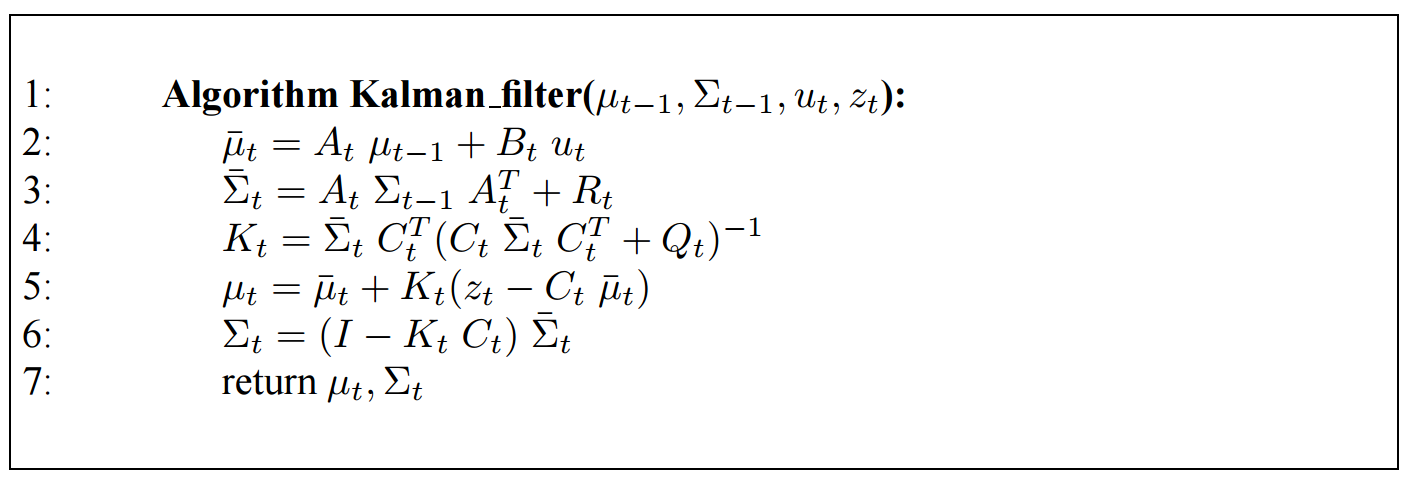
\includegraphics[width=1\textwidth]{billeder/KalmanFilter.png}
\caption{Kalman Filter algorithm}
\label{fig:kalmanfilter}
\end{figure}
If we look at the math, we can see that this can be done in a few steps. looking at the equations of the kalman filter we normally call 2-3 for the prediction step and 4-7 for the measurement step. 
\subsubsection{Prediction Step}
Looking at the equations in the prediction step (\ref{Pre1}, \ref{Pre2}).
\begin{gather}
\overline{\mu}_t = A_t \mu_{t-1} + B_t u_t
\label{Pre1}\\
\overline{\Sigma}_t = A_t \Sigma_{t-1} A^{\intercal}_t+ R_t
\label{Pre2}
\end{gather}
There are 2 conversion matrices $A$, $B$ and a measurement/input matrix $u$. The matrix $A$ must transform the last best estimate to the current domain. e.g. if we are trying to predict how far down a bungee jumper have fallen then the $A$ matrix must add the distance the gravity would have pulled him down since the last estimate $\mu_{t-1}$. We call this the static influence, since it is the change in the system if we do not interfere. The input matrix $u$ is the change we put in to the system since the last prediction. Lets say that we can increase or decrease the bungee jumpers air resistance. The $u$ matrix will contain the information about the change in air resistance. The $B$ matrix will convert the input matrix to the desired domain. For the bungee jumper it will convert air resistance to a fall distance. We call this the dynamic influence.
The last matrix $R$ is the noise, expressed as the covariance, of the input matrix $u$. This is to inform the system about the certainty of the input. 

As previously mentioned this dictates that there exists a linear conversion from the static and dynamic influences in relation to the the previous state to the new state. 
\subsubsection{Measurement Step}
Looking at the equations in the measurement step (\ref{Mes1}, \ref{Mes2} , \ref{Mes3}).
\begin{gather}
K_t = \overline{\Sigma}_t C^{\intercal}_t ( C_t \overline{\Sigma}_t C^{\intercal}_t + Q_t ) ^{-1} 
\label{Mes1} \\
\mu_{t} = \overline{\mu}_t +K_t (z_t-C_t\overline{\mu}_t) 
\label{Mes2} \\
\Sigma_t = (I-K_t C_t) \overline{\Sigma}_t 
\label{Mes3}
\end{gather}
The measurement step takes the predicted value $\overline{\mu}_t$, $\overline{\Sigma}_t$ and uses the measurement to fix the error in the prediction introduced by the noise. The measurement vector $z_t$ contains the measurement. For the bungee jumper it could be the tension in the bungee line. The conversion matrix $C_t$ convert the measurement to the value domain. So it takes the tension and convert to a distance. The $Q_t$ matrix is our measurement noise, expressed as the covariance.

By calculating the Kalman gain $K_t$ we get a kind of believe on the measurement, that decides how much we are able to affect the predicted value with information obtained from the measurement. 

After we have corrected the prediction, we have the best possible guess of the true value, or the true distance in the bungee case. 
\subsubsection{Graphical}
Looking at the bungee example, this can also be graphically shown. On figure \ref{bungeeFig} we see the bungee problem. 
\begin{figure}[H]
\centering
\includegraphics[width=1\textwidth]{billeder/Bungee.jpg}
\caption{The bungee problem}
\label{bungeeFig}
\end{figure}
First we see a the prediction step which have a very high uncertainty as shown with a Gaussian with a big variance. After this we make a measurement, as show in the second graph. we now use the kalman filter to estimate the best guess, based on the prediction and the measurement. 

We can see this as optimal fusion of our prediction information and our measurement information. 
\subsubsection{Kalman Filters In Robotics}
Like in the bungee example where the position of the bungee jumper was found. A robot can be located in a known map. 
But this is not the only use of a kalman filters in robotics.\\
Kalman filters are often used to fuse multiple sensor readings to one optimal guess, and to discover hidden variables. A hidden variable is a property that can not be directly measured, but have a relation to the measured data. lets say you can measure the location of a robot. Then the hidden variable can be the robots speed since the speed can be found looking at different locations over time. By using a kalman filter it is possible to estimate the speed very precise. \\
Since the kalman filter is uni-model, which mean that it only can give one guess of the location, other techniques, like particle filters and Markov localisation which gives multiple candidate locations, are often preferred. 
\subsubsection{Extended Kalman Filter}
One of the big limitations of the kalman filter is the requirement that dictates that there must be a linear relationship between measurements or input and the value domain. 

This limitation is removed in the extended kalman filter. This is done by replacing the linear conversion matrices $A$, $B$ and $C$ with the none linear functions $g(u_t, \mu_{t-1})$ and $h(\overline{\mu}_t)$.\\

Since the kalman filter basically exploits the principle of a Gaussian converted with a linear transformation still is a Gaussian. Introducing the non linear functions brakes the filter. To fix this the extended kalman filter utilize a method called first order Taylor expansion. Taylor expansion construct a linear approximation to a function, in a given point. This is done by using the partial derivative of the function in the point. We create the partial derivative matrices $G$ and $H$.
\begin{equation}
G = \frac{\partial g(u_t, \mu_{t-1})}{\partial \mu_{t-1}} \\ H = \frac{\partial h(\overline{\mu}_t)}{\partial \overline{\mu}}
\end{equation}
We can now use this in the regular kalman filter to obtain the extended kalman filter.
\begin{figure}[H]
\centering
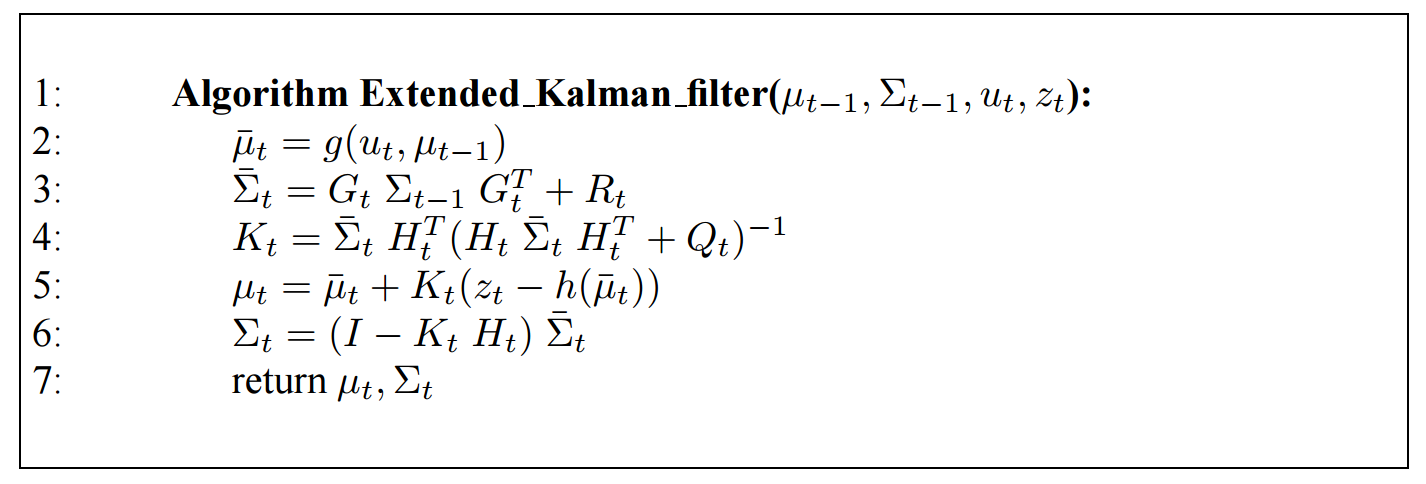
\includegraphics[scale=0.51]{billeder/EKF.png}
\caption{Extended Kalman Filter algorithm}
\end{figure}
It has been shown that this type of kalman filter is far better in practice than the regular kalman filter if the variance of prediction and measurement is small. If this is not the case the linearisation introduces additional noise. This is due to the error between the linearisation and the true function. The greater the variance the greater impact it has.  
